\documentclass[11pt]{article}
\usepackage{amsmath}
\usepackage{amssymb}
\usepackage{amsthm}
\usepackage{amscd}
\usepackage{amsfonts}
\usepackage{graphicx}%
\usepackage{fancyhdr}
\usepackage{color}
\usepackage{cite}

%\usepackage[T1]{fontenc}
\usepackage[utf8]{inputenc}
\usepackage{authblk}
\usepackage{physics}
\usepackage{float}
\usepackage{caption}
\usepackage{subcaption}
\newcommand{\expv}[1]{\ensuremath{\mathbb{E}[ #1]}}
\newcommand{\xs}[2]{\ensuremath{\Sigma_{#1}^{(#2)}}}
\newcommand{\intO}{\ensuremath{\int\limits_{4\pi}}}
\newcommand{\intz}{\ensuremath{\int\limits_0^1}}
\newcommand{\intf}{\ensuremath{\int\limits_{-\infty}^\infty}}
\newcommand{\intzf}{\ensuremath{\int\limits_{0}^\infty}}
\newcommand{\LargerCdot}{\raisebox{-0.25ex}{\scalebox{1.2}{$\cdot$}}}

\textwidth6.6in
\textheight9in


\setlength{\topmargin}{0.3in} \addtolength{\topmargin}{-\headheight}
\addtolength{\topmargin}{-\headsep}

\setlength{\oddsidemargin}{0in}

\oddsidemargin  0.0in \evensidemargin 0.0in \parindent0em

%\pagestyle{fancy}\lhead{MATH 579 (UQ for PDEs)} \rhead{02/24/2014}
%\chead{Project Proposal} \lfoot{} \rfoot{\bf \thepage} \cfoot{}


\begin{document}

\title{HDMR and SC on SG \\for an Analytic Problem}

\author[]{Paul Talbot\thanks{talbotp@unm.edu}}
%\date{}
\renewcommand\Authands{ and }
\maketitle
\newpage
\section{Approximations}
We use the sparse grid approximation for stochastic collocation described elsewhere,
\begin{equation}
u(Y)\approx S[u](Y)\equiv \sum_{\vec i\in\Lambda(L)} S^i[u](Y),
\end{equation}
\begin{equation}
 S^i[u](Y) = c(\vec i)\bigotimes_{n=1}^N U[u](Y),
\end{equation}
\begin{equation}
c(\vec i)\equiv \sum_{\vec j\in\{0,1\}^N,\hspace{5pt}\vec j+\vec i \in \Lambda} (-1)^{|\vec j|_1},
\end{equation}
\begin{equation}
\bigotimes_{n=1}^N U[u](Y)\equiv \sum_{\vec k}^{\vec i} u_h(Y^{(\vec k)}) L_{\vec k}(Y).
\end{equation}
Further, we apply a Cut-HDMR representation, where
\begin{equation}
u(Y)= u_0 + \sum_i^N u_i + \sum_i^N\sum_j^i u_{i,j}+...,
\end{equation}
\begin{equation}
u_0=u(\bar Y)
\end{equation}
\begin{equation}
u_i\equiv u(Y_i,\bar Y),
\end{equation}
\begin{equation}
u_{i,j}\equiv u(Y_i,Y_j,\bar Y),
\end{equation}
and so on.  Here $N$ is the total number of uncertain inputs, and $\bar Y$ indicates holding any variables not explicitly listed at a reference value (in this case, the mean value).  This cut-HDMR representation allows us to approximate by truncating at a particular interaction level $H$.  For instance, an $H2$ approximation would only include the terms
\begin{equation}
u(Y)\approx H_2[u](Y) = u_0 + \sum_i^N u_i + \sum_i^N\sum_j^{i-1} u_{i,j}.
\end{equation}
We combine the two by using SC on SG to evaluate the HDMR terms.  For example,
\begin{equation}
u(Y)\approx H_2[u](Y)\approx S_0 + \sum_i^N S_i + \sum_i^N\sum_j^{i-1} S_{i,j},
\end{equation}
\begin{equation}
S_0\equiv S[u](\bar Y),
\end{equation}
\begin{equation}
S_i\equiv S[u](Y_i,\bar Y),
\end{equation}
\begin{equation}
S_{i,j}\equiv S[u](Y_i,Y_j,\bar Y).
\end{equation}

\section{Problem}
The problem we are applying uncertainty to is equivalent to the flux of particles emitted through multiple equally-spaced purely-absorbing materials with a source on the opposite side.  The general solution to such a system is
\begin{equation}
u(\Sigma) = A\prod_i^N e^{-\Sigma_i x_i},
\end{equation}
where $A$ is the initial source strength, $\Sigma_i$ is the macroscopic interaction cross section, and $x_i$ is the width of the material.  Assuming all materials are equal in size and the initial source is unity, we can normalize to obtain the general solution
\begin{equation}
u(Y) = \prod_i^N e^{-Y_i}=e^{-\sum_i^N Y_i}.
\end{equation}
The expected value of $u(Y)$ is
\begin{equation}
\expval{u(Y)} = \int_a^b u(Y)P(Y)dY,
\end{equation}
where $P(Y)$ is the joint-pdf of the combined uncertainty space of $Y$.  In our case, we will assume $Y_n$ are distributed uniformly from $1$ to $6$.  The joint PDF for this independent inputs is 
\begin{equation}
P(Y)=5^{-N}.
\end{equation}

\subsection{Cases}
We consider four distinct cases, varying the number of uncertain variable inputs as $N\in(5,10,15,30)$.  For each case, we will compare analog Monte Carlo uncertainty quantification with direct stochastic collocation on sparse grids as well as cut-HDMR for truncation levels $H\in(1,2,3)$.  For each case, we increase the level $L$ of the sparse grid expansion and plot the resulting error in the expected value of $u(Y)$ as a function of total deterministic solver runs.  This effectively produces a comparison of error obtained by computational cost.  For clarity, the approximations made are
\begin{itemize}
\item $L$, the ``level'' of sparse grid approximation, used to produce quadrature points;
\item $H$, the HDMR truncation level,
\item TD, HDMR, or MC for (total degree) stochastic collocation, HDMR, or MC sampling methods.
\end{itemize}

\subsection{Results}
\begin{figure}[H]
\centering
  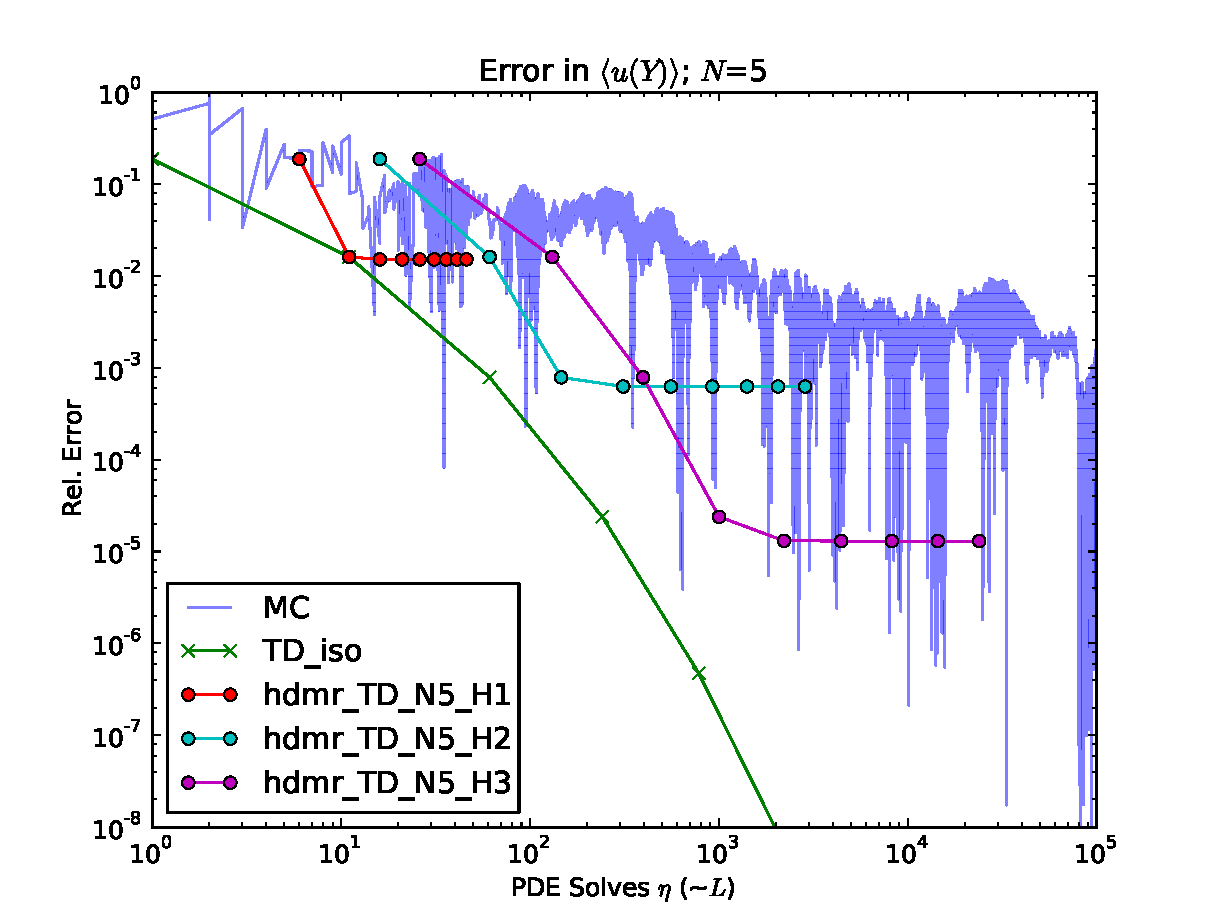
\includegraphics[width=0.7\linewidth]{hdmrN5}
  \caption{$N=5$}
  \label{geom}
\end{figure}
\begin{figure}[H]
\centering
  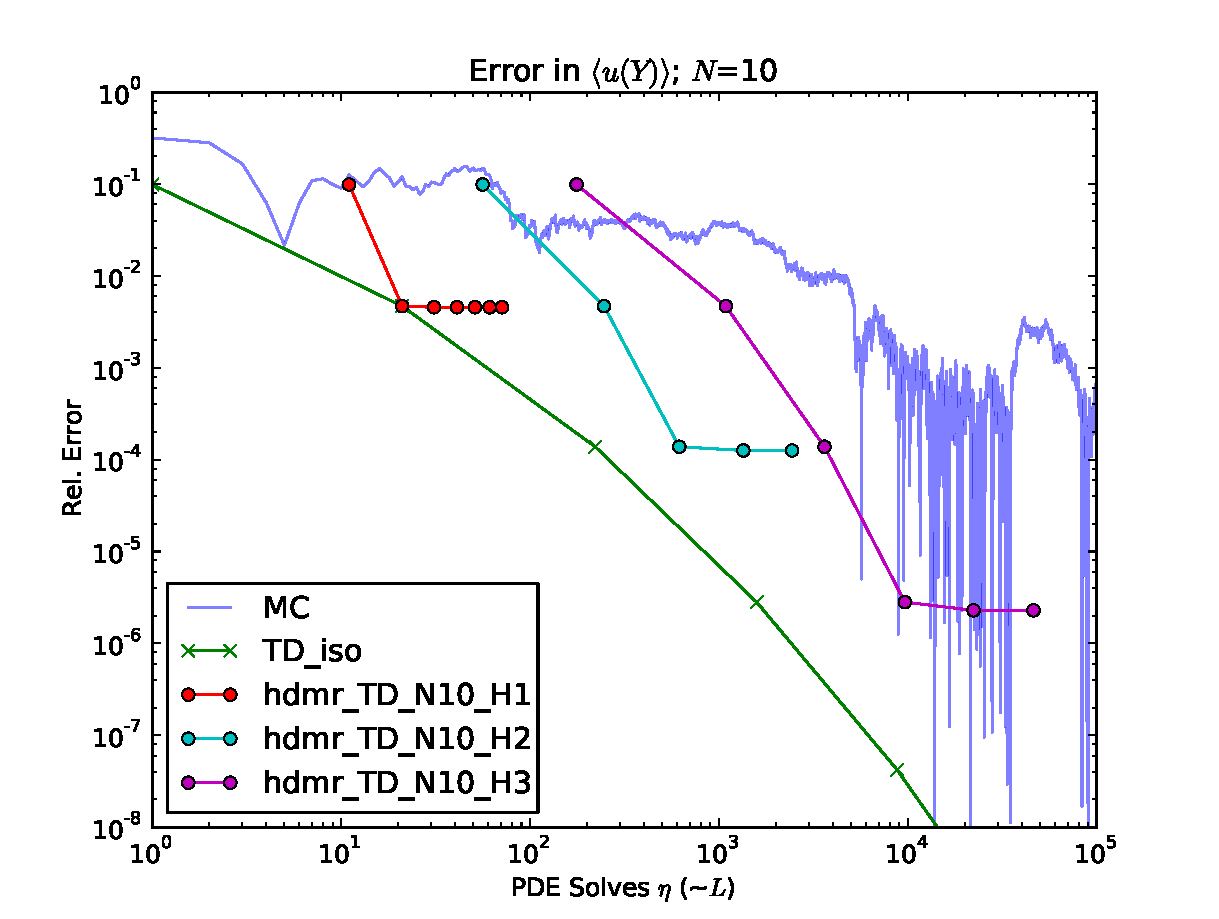
\includegraphics[width=0.7\linewidth]{hdmrN10}
  \caption{$N=10$}
  \label{geom}
\end{figure}
\begin{figure}[H]
\centering
  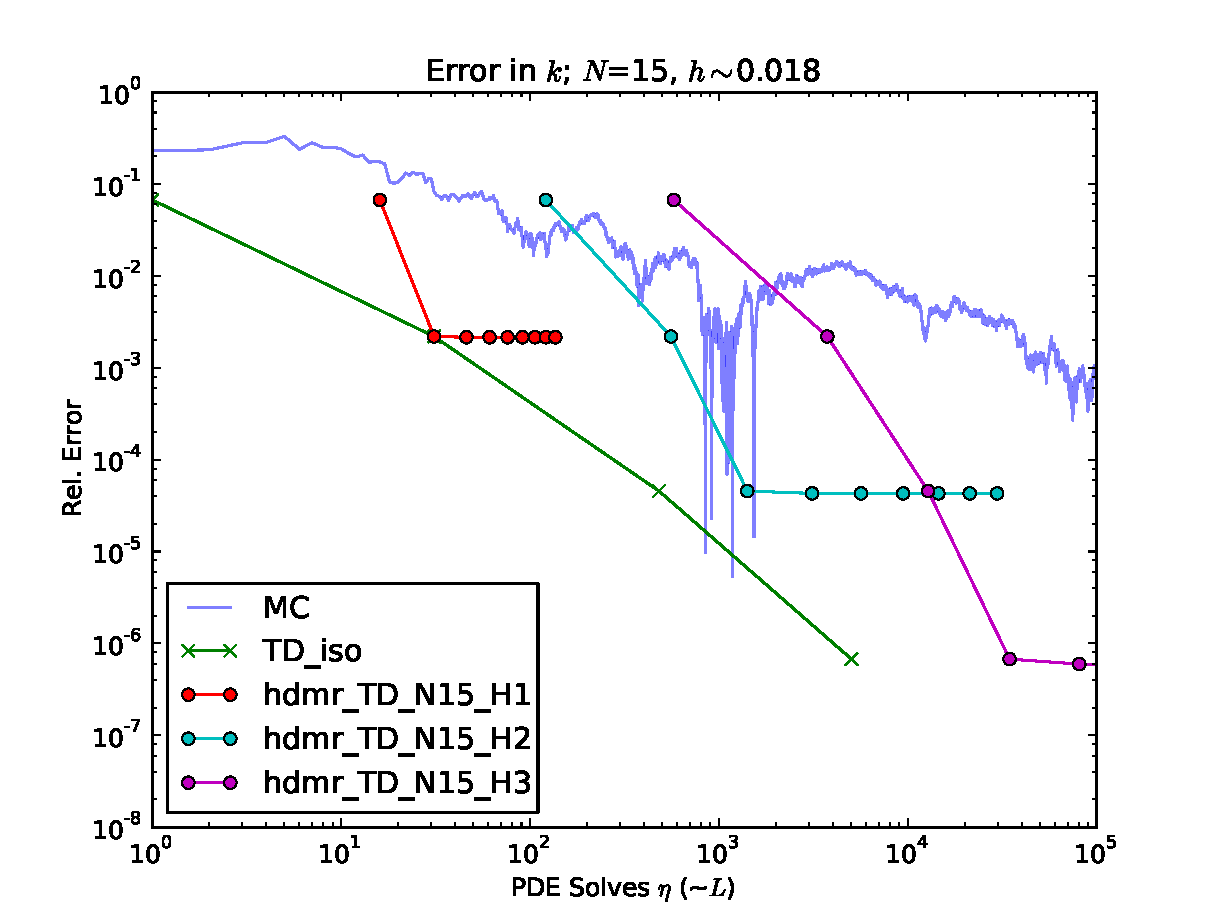
\includegraphics[width=0.7\linewidth]{hdmrN15}
  \caption{$N=15$}
  \label{geom}
\end{figure}
\begin{figure}[H]
\centering
  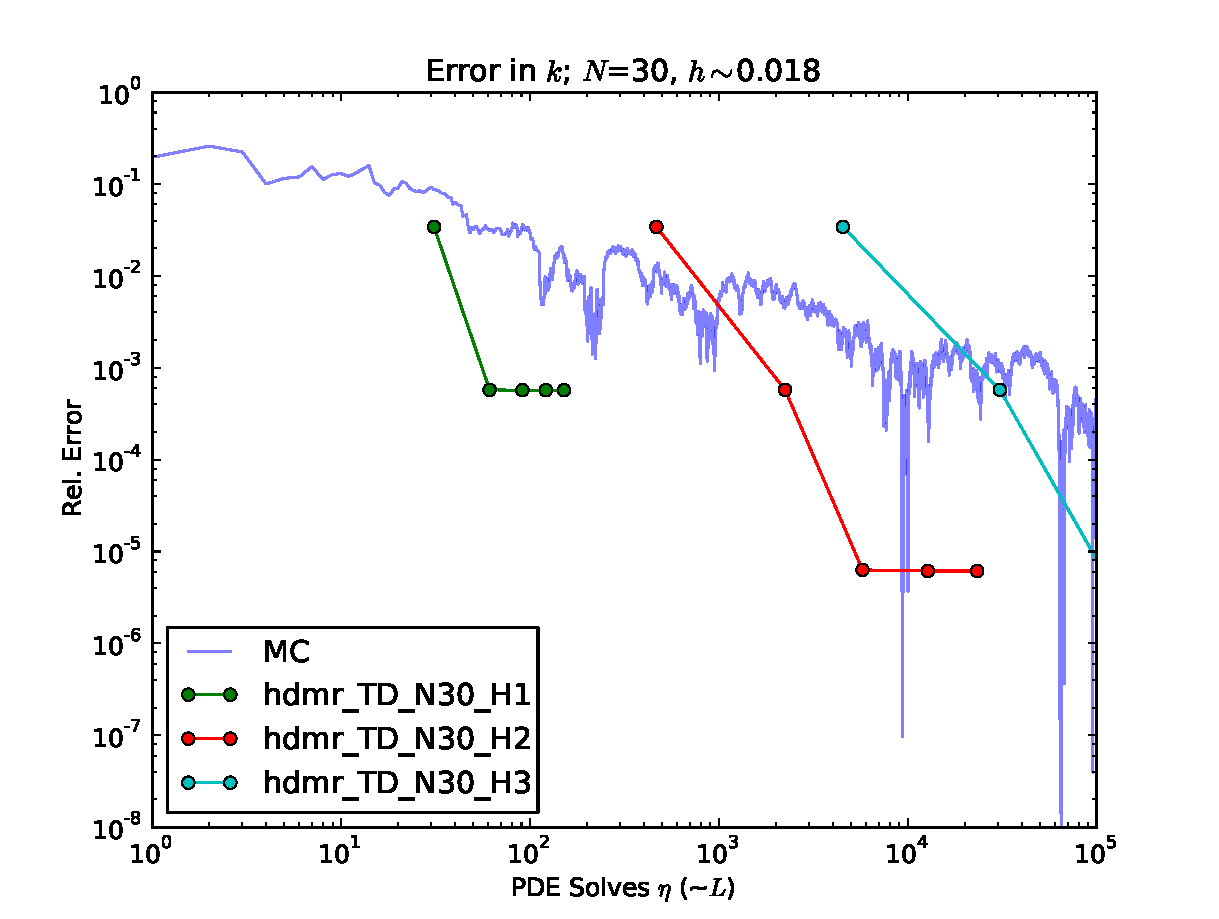
\includegraphics[width=0.7\linewidth]{hdmrN30_inc}
  \caption{$N=30$}
  \label{geom}
\end{figure}

\end{document}